% Auto-generated by recursive_marker_transformer.mor_tables -- do not edit.
\section{Reproduction of the Mixture-of-Recursions tables on the genomap suite}
We reproduce every table of the Mixture-of-Recursions paper (Bae et al., 2025) with SMART on the genomap single-cell datasets (and the pathway/P-NET multi-omics cohorts), with no TCGA. Each table below names the MoR table(s) it reproduces and the claim it supports (adaptive recursion loop, token reduction, or parameter reduction). Cells are macro-F1 (mean$\pm$std over seeds where available).
\paragraph{Adaptive depth.} SMART's core adaptive-computation result. Single-pass (K=1), fixed-depth recursion, and adaptive per-token routed depth (expert-choice MoR) are compared; mean token depth and compute-saved quantify the funnel -- uninformative marker tokens exit early, cutting recursion FLOPs while tracking fixed-depth accuracy..
\begin{table}[htbp]\centering\footnotesize
\setlength{\tabcolsep}{4pt}
\caption{Adaptive depth: K=1 (no recursion) vs fixed-depth vs adaptive routed depth (MoR's core claim).}
\label{tab:mor-adaptive}
\resizebox{\ifdim\width>\linewidth\linewidth\else\width\fi}{!}{%
\begin{tabular}{lrrrrr}
\toprule
Dataset & K=1 (no recursion) & fixed depth K & adaptive depth (MoR) & mean token depth & compute saved \\
\midrule
tabula\_muris & 73.1 & 77.1 & 72.7 & 2.75/4 & 31\% \\
pancreas & 51.7 & 53.6 & 53.5 & 2.75/4 & 31\% \\
common\_class & 66.2 & 68.5 & 66.2 & 2.75/4 & 31\% \\
prototype & 93.2 & 94.1 & 94.2 & 2.75/4 & 31\% \\
baron & 57.5 & 65.8 & 64.5 & 2.75/4 & 31\% \\
segerstolpe & 7.7 & 9.8 & 5.9 & 2.75/4 & 31\% \\
\bottomrule
\end{tabular}
}
\end{table}
\paragraph{T3 / T7.} MoR Tables 3 and 7. Macro-F1 of Vanilla (K independent blocks), Recursive (one shared block applied K times), and MoR (shared block + expert-choice routing) across four model sizes -- Recursive matches Vanilla at about 1/K the parameters..
\begin{table}[htbp]\centering\footnotesize
\setlength{\tabcolsep}{4pt}
\caption{T3 / T7: MoR vs Recursive vs Vanilla across model sizes.}
\label{tab:mor-t3}
\resizebox{\ifdim\width>\linewidth\linewidth\else\width\fi}{!}{%
\begin{tabular}{lrrrrrr}
\toprule
Arch x size (macro\_f1) & tabula\_muris & pancreas & common\_class & prototype & baron & segerstolpe \\
\midrule
Vanilla (independent) d=48 & 74.5 & 51.1 & 78.8 & 95.5 & 69.8 & 7.3 \\
Vanilla (independent) d=96 & 78.0 & 55.5 & 71.7 & 94.7 & 64.5 & 9.8 \\
Vanilla (independent) d=192 & 78.0 & 56.8 & 3.0 & 96.2 & 3.3 & 9.2 \\
Vanilla (independent) d=384 & 52.4 & 5.3 & 3.0 & 76.3 & 3.3 & 5.9 \\
Recursive (shared) d=48 & 73.7 & 54.3 & 77.6 & 94.3 & 67.0 & 6.6 \\
Recursive (shared) d=96 & 73.5 & 58.1 & 70.6 & 94.2 & 65.6 & 8.6 \\
Recursive (shared) d=192 & 79.7 & 61.5 & 62.1 & 95.2 & 59.7 & 7.0 \\
Recursive (shared) d=384 & 0.5 & 53.8 & 23.0 & 74.2 & 16.4 & 6.4 \\
MoR (SMART) d=48 & 68.7 & 57.8 & 75.6 & 93.5 & 67.6 & 4.8 \\
MoR (SMART) d=96 & 71.9 & 56.7 & 68.6 & 93.3 & 60.3 & 5.9 \\
MoR (SMART) d=192 & 74.0 & 65.6 & 61.5 & 95.3 & 62.4 & 10.0 \\
MoR (SMART) d=384 & 65.8 & 53.4 & 42.8 & 91.6 & 60.1 & 9.9 \\
\bottomrule
\end{tabular}
}
\end{table}
\paragraph{T4.} MoR Table 4 (the headline router ablation). Expert- vs token-choice routing and the marker-selection baselines (random/variance) vs the learned router; mean+-std over seeds across the genomap suite..
\begin{table}[htbp]\centering\footnotesize
\setlength{\tabcolsep}{4pt}
\caption{T4: expert/token-choice router + marker-selection ablation.}
\label{tab:mor-t4}
\resizebox{\ifdim\width>\linewidth\linewidth\else\width\fi}{!}{%
\begin{tabular}{lrrrrrr}
\toprule
Variant (macro-F1) & tabula\_muris & pancreas & common\_class & prototype & baron & segerstolpe \\
\midrule
expert-choice MoR (shared) & 72.7$\pm$1.1 & 53.5$\pm$1.1 & 66.2$\pm$2.9 & 94.2$\pm$0.4 & 64.5$\pm$0.0 & 5.9$\pm$0.0 \\
token-choice MoR & 75.1$\pm$2.1 & 58.7$\pm$5.3 & 67.4$\pm$3.4 & 94.3$\pm$0.6 & 58.6$\pm$0.0 & 5.5$\pm$0.0 \\
fixed-depth (no routing) & 77.1$\pm$2.1 & 53.6$\pm$1.6 & 68.5$\pm$2.7 & 94.1$\pm$0.3 & 65.8$\pm$0.0 & 9.8$\pm$0.0 \\
K=1 (no recursion) & 73.1$\pm$2.4 & 51.7$\pm$5.2 & 66.2$\pm$3.7 & 93.2$\pm$0.5 & 57.5$\pm$0.0 & 7.7$\pm$0.0 \\
independent blocks & 75.5$\pm$0.8 & 57.3$\pm$1.9 & 66.6$\pm$4.4 & 94.2$\pm$0.4 & 58.3$\pm$0.0 & 7.0$\pm$0.0 \\
random markers & 74.6$\pm$3.1 & 59.0$\pm$2.0 & 63.6$\pm$3.9 & 96.8$\pm$0.0 & 65.5$\pm$0.0 & 5.5$\pm$0.0 \\
variance markers & 75.6$\pm$0.7 & 59.2$\pm$2.3 & 72.2$\pm$1.8 & 95.4$\pm$0.6 & 73.3$\pm$0.0 & 9.6$\pm$0.0 \\
\bottomrule
\end{tabular}
}
\end{table}
\paragraph{T6.} MoR Table 6. Parameter counts of the size variants and the MoR-vs-Vanilla reduction factor (about K, from weight sharing)..
\begin{table}[htbp]\centering\footnotesize
\setlength{\tabcolsep}{4pt}
\caption{T6: model-size config + parameter reduction (MoR vs Vanilla params).}
\label{tab:mor-t6}
\resizebox{\ifdim\width>\linewidth\linewidth\else\width\fi}{!}{%
\begin{tabular}{lrrrr}
\toprule
Size & Recursions & MoR params & Vanilla params & param reduction \\
\midrule
d\_model=48 & K=4 & 19,152 & 75,840 & 4.0$\times$ \\
d\_model=96 & K=4 & 75,168 & 299,136 & 4.0$\times$ \\
d\_model=192 & K=4 & 297,792 & 1,188,096 & 4.0$\times$ \\
d\_model=384 & K=4 & 1,185,408 & 4,735,488 & 4.0$\times$ \\
\bottomrule
\end{tabular}
}
\end{table}
\paragraph{T1 / T5 / T8.} MoR Tables 1, 5, 8. The four parameter-sharing schemes (Cycle, Sequence, Middle-Cycle, Middle-Sequence) at K=6 with three unique blocks, bracketed by the fully-shared (1 block) and fully-independent (6 blocks) extremes..
\begin{table}[htbp]\centering\footnotesize
\setlength{\tabcolsep}{4pt}
\caption{T1 / T5 / T8: parameter-sharing schemes (Cycle/Sequence/Middle-*).}
\label{tab:mor-t1}
\resizebox{\ifdim\width>\linewidth\linewidth\else\width\fi}{!}{%
\begin{tabular}{lrrrrrrr}
\toprule
Sharing scheme (K=6) & params & tabula\_muris & pancreas & common\_class & prototype & baron & segerstolpe \\
\midrule
shared (1 block) & 74,784 & 75.1 & 61.0 & 68.9 & 93.6 & 60.2 & 3.4 \\
Cycle (3) & 224,352 & 80.5 & 54.4 & 71.6 & 95.2 & 70.5 & 6.9 \\
Sequence (3) & 224,352 & 78.5 & 57.6 & 0.8 & 93.9 & 66.1 & 4.5 \\
Middle-Cycle (3) & 224,352 & 80.1 & 56.4 & 67.0 & 94.9 & 61.0 & 7.8 \\
Middle-Sequence (3) & 224,352 & 80.1 & 56.4 & 67.0 & 94.9 & 61.0 & 7.8 \\
independent (6) & 448,704 & 79.9 & 57.0 & 3.0 & 95.4 & 65.3 & 7.2 \\
\bottomrule
\end{tabular}
}
\end{table}
\paragraph{T2 / T12 / T13.} MoR Tables 2, 12, 13 (adapted to a non-autoregressive set encoder). Step-cache: reusing the step-1 attention key/value across recursions vs recomputing -- the analogue of MoR's recursion-wise KV-cache sharing..
\begin{table}[htbp]\centering\footnotesize
\setlength{\tabcolsep}{4pt}
\caption{T2 / T12 / T13: step-cache: reuse vs recompute step-1 K/V.}
\label{tab:mor-t2}
\resizebox{\ifdim\width>\linewidth\linewidth\else\width\fi}{!}{%
\begin{tabular}{lrrrrrr}
\toprule
KV strategy (macro-F1) & tabula\_muris & pancreas & common\_class & prototype & baron & segerstolpe \\
\midrule
recompute K/V (no cache) & 79.9 & 54.1 & 70.4 & 93.9 & 65.6 & 8.6 \\
reuse step-1 K/V (step-cache) & 71.6 & 58.5 & 71.8 & 93.2 & 59.6 & 6.4 \\
\bottomrule
\end{tabular}
}
\end{table}
\paragraph{T9.} MoR Table 9 (adapted). Warm-start / uptraining: a MoR model whose shared block is initialised from a trained fixed-depth model, vs trained from scratch..
\begin{table}[htbp]\centering\footnotesize
\setlength{\tabcolsep}{4pt}
\caption{T9: warm-start (uptraining analogue: fixed-depth source -> MoR).}
\label{tab:mor-t9}
\resizebox{\ifdim\width>\linewidth\linewidth\else\width\fi}{!}{%
\begin{tabular}{lrrrrrr}
\toprule
Warm-start (macro-F1) & tabula\_muris & pancreas & common\_class & prototype & baron & segerstolpe \\
\midrule
fixed-depth source & 75.2 & 51.8 & 69.0 & 92.9 & 68.1 & 8.3 \\
MoR from scratch & 71.7 & 62.8 & 65.8 & 95.5 & 61.5 & 5.4 \\
MoR warm-started & 65.8 & 61.6 & 64.8 & 93.3 & 55.8 & 6.9 \\
warm-start gain & -5.9 & -1.2 & -0.9 & -2.2 & -5.6 & +1.5 \\
\bottomrule
\end{tabular}
}
\end{table}
\paragraph{T10 / T11.} MoR Tables 10 and 11. Expert- and token-choice routers under different routing configurations (linear vs MLP router head, temperature, load balancing)..
\begin{table}[htbp]\centering\footnotesize
\setlength{\tabcolsep}{4pt}
\caption{T10 / T11: expert/token router under different routing configs.}
\label{tab:mor-t10}
\resizebox{\ifdim\width>\linewidth\linewidth\else\width\fi}{!}{%
\begin{tabular}{lrrrrrr}
\toprule
Routing config (macro-F1) & tabula\_muris & pancreas & common\_class & prototype & baron & segerstolpe \\
\midrule
expert linear & 71.9 & 56.7 & 68.6 & 93.3 & 60.3 & 5.9 \\
expert MLP & 67.2 & 51.9 & 70.2 & 93.2 & 49.4 & 7.1 \\
expert temp=2 & 73.5 & 57.6 & 66.7 & 94.1 & 66.2 & 6.5 \\
token linear & 74.7 & 53.7 & 70.1 & 94.5 & 52.6 & 5.4 \\
token MLP & 78.8 & 59.7 & 64.4 & 94.0 & 60.9 & 5.5 \\
token balance=0.01 & 75.6 & 57.6 & 67.5 & 93.7 & 58.6 & 5.0 \\
\bottomrule
\end{tabular}
}
\end{table}
\paragraph{T14 / Fig5.} MoR Table 14 / Figure 5. Per-marker recursion depth and the fraction of marker tokens still active at each recursion step (the compute-allocation funnel)..
\begin{table}[htbp]\centering\footnotesize
\setlength{\tabcolsep}{4pt}
\caption{T14 / Fig5: per-marker recursion depth + active-fraction-per-step.}
\label{tab:mor-t14}
\resizebox{\ifdim\width>\linewidth\linewidth\else\width\fi}{!}{%
\begin{tabular}{lrr}
\toprule
Dataset & mean token depth & active fraction per step (1..K) \\
\midrule
tabula\_muris & 2.75/4 & 1.00, 0.75, 0.50, 0.50 \\
pancreas & 2.75/4 & 1.00, 0.75, 0.50, 0.50 \\
common\_class & 2.75/4 & 1.00, 0.75, 0.50, 0.50 \\
prototype & 2.75/4 & 1.00, 0.75, 0.50, 0.50 \\
baron & 2.75/4 & 1.00, 0.75, 0.50, 0.50 \\
segerstolpe & 2.75/4 & 1.00, 0.75, 0.50, 0.50 \\
\bottomrule
\end{tabular}
}
\end{table}
\paragraph{Pathway data.} The new GitHub P-NET/Reactome multi-omics cohorts run through the same architecture ablation, showing the three claims transfer beyond genomap to bulk mutation/CNV/expression data..
\begin{table}[htbp]\centering\footnotesize
\setlength{\tabcolsep}{4pt}
\caption{Pathway data: GitHub P-NET/Reactome cohorts through the architecture ablation.}
\label{tab:mor-pathway}
\resizebox{\ifdim\width>\linewidth\linewidth\else\width\fi}{!}{%
\begin{tabular}{lrrrrrr}
\toprule
Pathway cohort (macro-F1) & prostate & blca & stad & brca & panmeta\_response & panmeta\_subtype \\
\midrule
adaptive MoR (shared) & 50.9 & 43.3 & 38.8 & 27.7 & 93.0 & 50.3 \\
independent & 47.5 & 40.4 & 55.3 & 28.8 & 91.8 & 34.2 \\
token-choice & 80.9 & 43.3 & 37.6 & 30.7 & 91.8 & 57.9 \\
fixed-depth & 75.5 & 43.3 & 36.4 & 22.6 & 91.5 & 68.4 \\
K=1 & 47.7 & 40.0 & 38.8 & 13.5 & 90.7 & 55.4 \\
\bottomrule
\end{tabular}
}
\end{table}
\begin{figure}[t]\centering
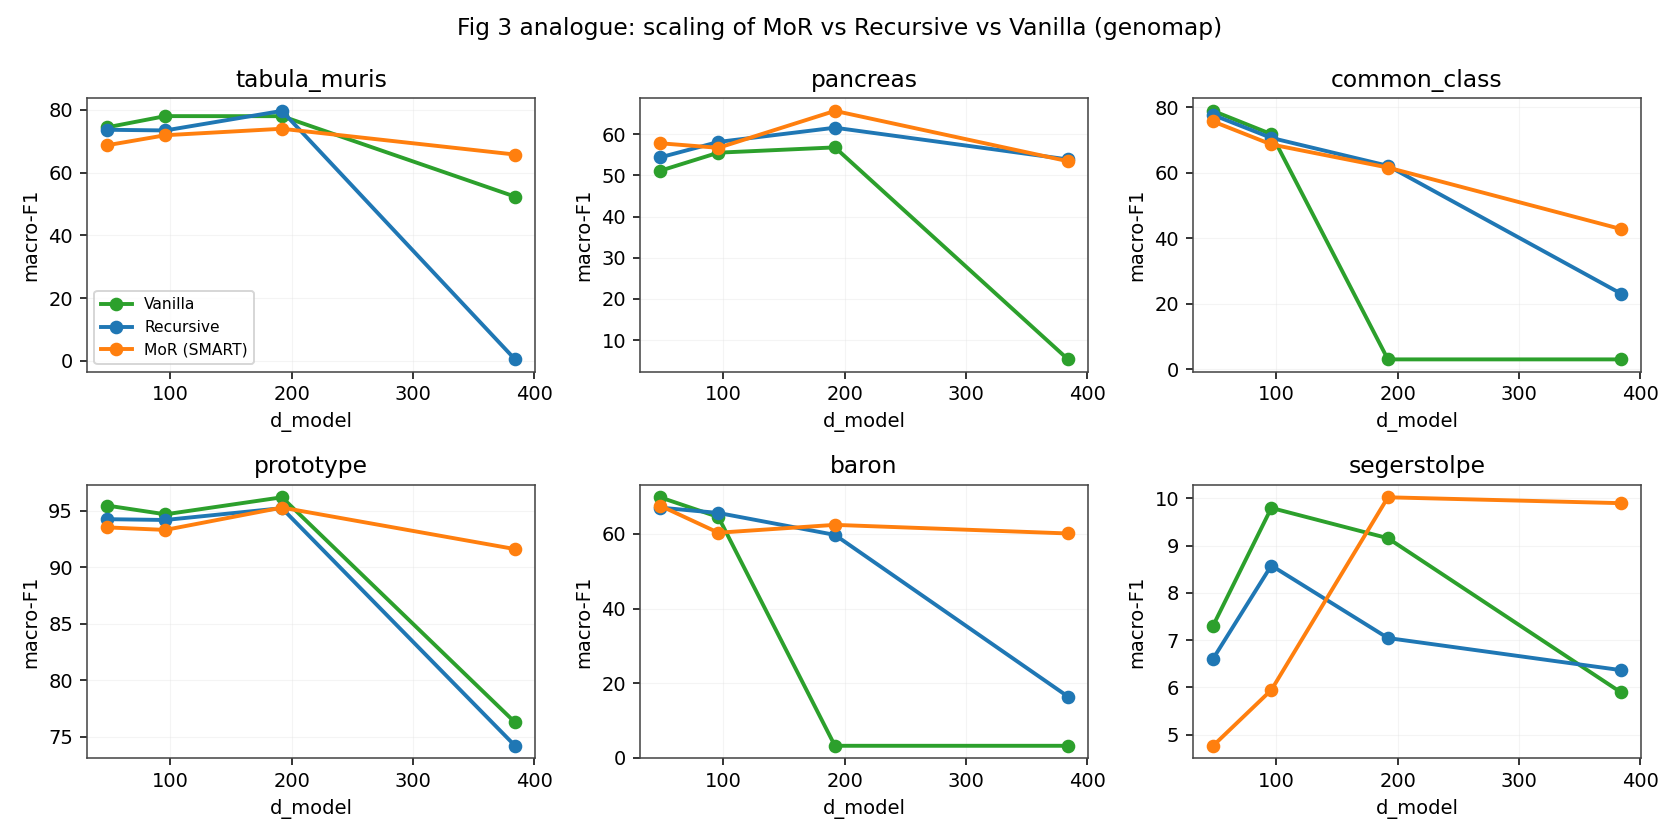
\includegraphics[width=0.9\linewidth]{figs/fig_scaling.png}
\caption{Fig 3 analogue: macro-F1 vs model size for Vanilla, Recursive and MoR on each genomap dataset.}
\label{fig:mor-scaling}
\end{figure}
\begin{figure}[t]\centering
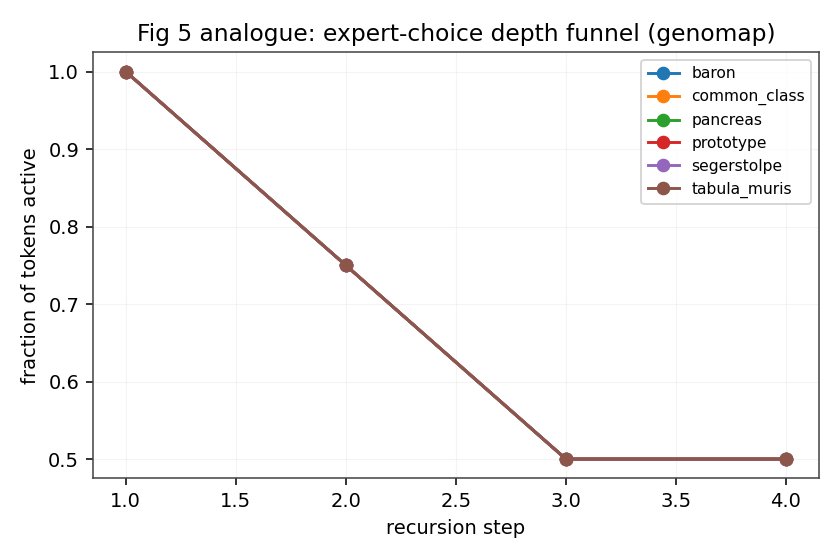
\includegraphics[width=0.9\linewidth]{figs/fig_depth.png}
\caption{Fig 5 analogue: fraction of marker tokens still active at each recursion step (the expert-choice depth funnel).}
\label{fig:mor-depth}
\end{figure}
\begin{figure}[t]\centering
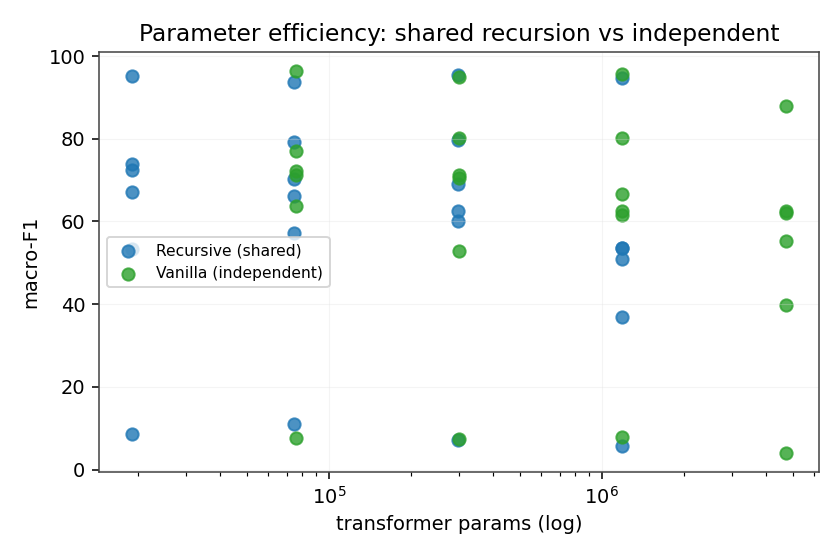
\includegraphics[width=0.9\linewidth]{figs/fig_param_efficiency.png}
\caption{Parameter efficiency: macro-F1 vs transformer parameters for shared-recursion vs independent stacks.}
\label{fig:mor-param}
\end{figure}
